\documentclass[10pt]{article}
\usepackage[paperwidth=210mm, paperheight=297mm, margin=0mm]{geometry}
\usepackage{tikz}
\usepackage{helvet}
\usepackage{xcolor}

\renewcommand{\familydefault}{\sfdefault}
\pagestyle{empty} 

% Colors
\definecolor{plannerbrown}{RGB}{180, 160, 140}
\definecolor{gridcolor}{RGB}{230, 225, 220}

\begin{document}

\begin{tikzpicture}[remember picture, overlay, shift={(current page.south west)}]
    
    % 1. BACKGROUND GRID (0.5cm steps)
    \draw[gridcolor, thin, step=0.5cm] (0,0) grid (21.0, 29.7);

    % 2. HEADER
    \node[anchor=west, font=\large\bfseries, text=plannerbrown] at (1.5, 28.15) {Date: \rule{6cm}{0.5pt}};
    % \node[anchor=east, font=\large\bfseries, text=plannerbrown] at (19.5, 28.8) {Page: \rule{1.5cm}{0.5pt}};

    % 3. REDUCED TOP BOX (10 lines)
    \draw[plannerbrown, thick] (1.5, 22.0) rectangle (19.5, 27.0);
    \foreach \l in {1,2,...,10} {
        \pgfmathsetmacro{\yTopLine}{27.0 - \l*0.5}
        \draw[plannerbrown, opacity=0.2, thin] (1.6, \yTopLine) -- (19.4, \yTopLine);
    }

    % 4. MAIN BOUNDARY 
    \draw[plannerbrown, thick] (1.5, 2.0) rectangle (19.5, 20.0);

    % 5. LEFT COLUMN: TIME TRACKING (6AM - 11PM)
    \foreach \h [count=\i] in {6,7,8,9,10,11,12,1,2,3,4,5,6,7,8,9,10,11} {
        \pgfmathsetmacro{\yHour}{20.0 - (\i-1)*1.0}
        
        % Hour Label
        \node[anchor=north west, font=\tiny\bfseries, text=plannerbrown] at (1.55, \yHour - 0.05) {\h};
        
        % Solid Hour Line
        \draw[plannerbrown, opacity=0.4] (1.5, \yHour) -- (6.5, \yHour);
        
        % Half-hour Line
        \pgfmathsetmacro{\yHalf}{\yHour - 0.5}
        \draw[plannerbrown, opacity=0.15] (1.5, \yHalf) -- (6.5, \yHalf);
    }

    % 6. WIDE RIGHT COLUMN (Notes / Tasks)
    \foreach \row in {1,...,36} {
        \pgfmathsetmacro{\yRow}{20.0 - \row*0.5}
        
        % CHECKBOX ALIGNMENT FIX:
        % Snapped to the 7.0cm grid line horizontally.
        % yRow is the bottom of the grid square; 0.1cm offset centers the 0.3cm box.
        \ifodd\row
            \draw[plannerbrown, opacity=0.5] (7.1, \yRow + 0.1) rectangle ++(0.3, 0.3);
        \fi
        
        % Task lines
        \draw[plannerbrown, opacity=0.2] (7.6, \yRow) -- (19.0, \yRow);
    }
    
    % 7. INTERNAL VERTICAL SEPARATOR
    \draw[plannerbrown, thin, dashed] (6.5, 2.0) -- (6.5, 20.0);

\end{tikzpicture}

\end{document}